% This is based on the LLNCS.DEM the demonstration file of
% the LaTeX macro package from Springer-Verlag
% for Lecture Notes in Computer Science,
% version 2.4 for LaTeX2e as of 16. April 2010
%
% See http://www.springer.com/computer/lncs/lncs+authors?SGWID=0-40209-0-0-0
% for the full guidelines.
%
\documentclass{llncs}
\usepackage{tikz}
\usepackage{pgfplots}
\usepackage{algorithm2e}
\usepackage{listings}
\usepackage{color}
\usepackage{hyperref}
\usepackage{geometry}
\geometry{
  a4paper,         % or letterpaper
  textwidth=15cm,  % llncs has 12.2cm
  textheight=24cm, % llncs has 19.3cm
  heightrounded,   % integer number of lines
  hratio=1:1,      % horizontally centered
  vratio=2:3,      % not vertically centered
}

\definecolor{dkgreen}{rgb}{0,0.6,0}
\definecolor{gray}{rgb}{0.5,0.5,0.5}
\definecolor{mauve}{rgb}{0.58,0,0.82}

\lstset{frame=tb,
  language=Java,
  aboveskip=3mm,
  belowskip=3mm,
  showstringspaces=false,
  columns=flexible,
  basicstyle={\small\ttfamily},
  numbers=none,
  numberstyle=\tiny\color{gray},
  keywordstyle=\color{blue},
  commentstyle=\color{dkgreen},
  stringstyle=\color{mauve},
  breaklines=true,
  breakatwhitespace=true,
  tabsize=3
}
\begin{document}


\title{Algor\'{i}tmica II. Algoritmos Metaheur\'{i}sticos}
%
\titlerunning{Enfriamiento Simulado}  % abbreviated title (for running head)
%                                     also used for the TOC unless
%                                     \toctitle is used
%
\author{Joaq\'{i}n Roiz Pagador\inst{1}}
%
\authorrunning{Ivar Ekeland et al.} % abbreviated author list (for running head)
%
%
\institute{Universidad Pablo de Olavide, Carretera Utrera s/n, Sevilla, Espa\~{n}a,\\
\email{quiniroiz@gmail.com}}

\maketitle              % typeset the title of the contribution

\begin{abstract}
El siguiente documento pertenece a una serie de documentos que pretende servir a modo de resumen para el temario de Algor\'{i}tmica II para el Grado en Ingenier\'{i}a Inform\'{a}tica en Sistemas de Informaci\'{o}n.\\
\keywords{algoritmos, metaheur\'{i}stica, enfriamiento, simulado, termodin\'{a}mica}
\end{abstract}
%
\section*{Enfriamiento Simulado.}
%
El enfriamiento simulado(SA) aplicado a los problemas de optimizaci\'{o}n emerge del trabajo de S. Kirkpatrick y V.Cerny. En la \'{e}poca de 1980, SA ha tenido un mayor impacto que las b\'{u}squedas heur\'{i}sticas debido a su simpleza y eficiencia solventando problemas de optimizaci\'{o}n combinacional. Ha sido extendido por su continua optimizaci\'{o}n de problemas.\\

SA se basa en el principio de mec\'{a}nica estad\'{i}stica donde se simula el proceso de enfriamiento lento que se aplica para obtener una estructura resistente de cristal.\\

Podemos basar el enfriamiento simulado como una simulaci\'{o}n de critalizaci\'{o}n que utiliza los fundamentos termodin\'{a}micos. Frente a los algoritmos cl\'{a}sicos presenta la mejora de que, a grandioso espacio a recorrer, no podremos asegurar un \'{o}ptimo global en un tiempo razonable.\\

Por tanto, utilizaremos tres estrategias posibles:
\begin{itemize}
\item Aceptar peores soluciones (Ref. Hill Climbing).
\item Modificar estructuras de entornos (de forma similar al caballo de ajedrez modificando sus posibles movimientos).
\item Comenzar b\'{u}squedas desde otras soluciones iniciales.
\end{itemize}

Nosotros utilizaremos la primera de ellas. \\

Sabremos el estado de la b\'{u}squeda hacia la soluci\'{o}n mediante un par\'{a}metro de control, que modela la funci\'{o}n de probabilidad. Disminuye as\'{i} la probabilidad de estos movimientos hacia soluciones peores.\\

La probabilidad de aceptaci\'{o}n disminuye conforme se va adelantando camino. \\

Referenciando a David D. de Vega: ''De forma similar a una b\'{u}squeda de mont\'{i}culos en un campo de f\'{u}tbol, nuestro algoritmo realizar\'{a} un barrido de sus vecinos en el punto que est\'{e} (mirar\'{a} a su alrededor). Llegado a un punto de probabilidad de aceptaci\'{o}n reducido, se le enviar\'{a} a otra parte del campo para buscar en otro punto diferente, de forma que podamos dar con un \'{o}ptimo local mejor y, tal vez, con el \'{o}ptimo global''. \\

Esta probabilidad se parametrizar\'{a} en temperatura (probabilidad de aceptaci\'{o}n para la soluci\'{o}n 'mala') y enfriamiento. Buscaremos por entoros por criterio de aceptaci\'{o}n, as\'{i} pues. \\

\subsection*{Caracter\'{i}sticas}

\begin{itemize}
\item M\'{e}todo de b\'{u}squeda por entornos caracterizado por un criterio de aceptaci\'{o}n de soluciones vecinas que var\'{i}a en tiempo de ejecuci\'{o}n.
\item Variables de entrada:
\begin{itemize}
\item Temperatura $\rightarrow$ En qu\'{e} medida se aceptar\'{a}n las soluciones vecinas 'peores'.
\begin{itemize}
\item $T_0 \rightarrow$ Valor alto, temperatura(T) inicial.
\item $T_f \rightarrow$ Condici\'{o}n de parada.
\end{itemize}
\item T se va reduciendo en cada iteraci\'{o}n (enfriamiento).
\end{itemize}
\item En cada iteraci\'{o}n se genera un n\'{u}mero de vecinos L(T)
\begin{itemize}
\item Pueden ser fijos siempre.
\item Depende de cada iteraci\'{o}n.
\end{itemize}
\item Cada vez que se genera un vecino, se aplica la probabilidad de aceptaci\'{o}n para ver si sustituye a la actual.
\begin{itemize}
\item Si la soluci\'{o}n vecina es mejor que la actual, se acepta autom\'{a}ticamente, como una b\'{u}squeda local cl\'{a}sica.
\item Si es peor, existe aun la probabilidad de que el vecino sustituya la soluci\'{o}n actual (Salir de \'{o}ptimos locales).
\end{itemize}
\end{itemize}

\begin{itemize}
\item Consideraciones de T:
\begin{itemize}
\item A mayor T, mayor probabilidad($P_a$) de soluciones peores (cuantas m\'{a}s iteraciones demos, menos soluciones peores aceptaremos).
\item Aceptar soluciones mucho peores al principio, pero no al final.
\end{itemize}
\item Consideraciones sobre $\delta$:
\begin{itemize}
\item A menor $\delta$, mayor $P_a$ de soluciones peores.
\item Tras cada iteraci\'{o}n se enfr\'{i}a la temperatura y se pasa a la siguiente iteraci\'{o}n.
\end{itemize}
\end{itemize}

A continuaci\'{o}n se listan las antolog\'{i}as al sistema de enfriamiento:\\

\begin{center}
\begin{tabular}{  c  c   }
  \hline
  Termodin\'{a}mica & SA\\ 
	\hline
  Estado del Sistema & Soluciones factibles \\
  Energ\'{i}a & Coste\\
  Cambios de estado & Soluci\'{o}n del entorno\\
  Temperatura & \textbf{Par\'{a}metro de control} \\
  Estado congelado & Soluci\'{o}n heur\'{i}stica\\
\end{tabular}
\end{center}

Resumiendo:

En cada iteraci\'{o}n, un vecino aleatorio es generado. Se comprobar\'{a} que el coste de la funci\'{o}n es siempre aceptado (mejor). En caso contrario, ser\'{a} seleccionado seg\'{u}n la probabilidad de aceptaci\'{o}n que depende de la temperatura y el total de su degradaci\'{o}n $\delta E$ de la funci\'{o}n objetivo. Este valor representa la diferencia del valor objetivo. En cada movimiento la probabilidad bajar\'{a}, por lo general representada de la siguiente forma:\\
\begin{center}
$P_a(\delta, T) = \epsilon^{-\frac{\delta}{T}}$
\end{center}

\begin{figure}
\begin{center}
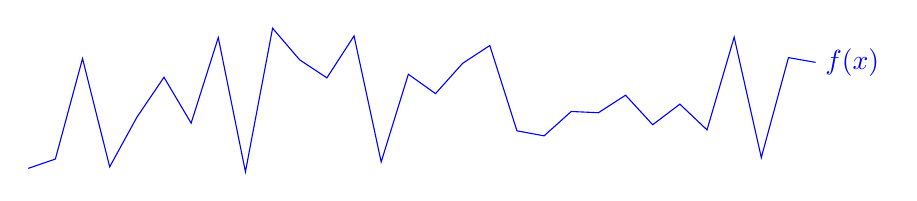
\begin{tikzpicture}
  \pgfmathsetseed{128}
  \draw[color=blue, samples=30] plot[domain=0:10] (\x,rand)
   node[right] {$f(x)$};
\end{tikzpicture}
\label{fig:Maximal3D}
\caption{Funci\'{o}n donde podemos observar diferentes \'{o}ptimos locales y uno global escondido entre ellos.}
\end{center}
\end{figure}

\begin{algorithm}[H]
\SetKwInOut{Input}{input}
\SetKwInOut{Output}{output}
\SetKwRepeat{Do}{do}{while}
    \Input{Cooling schedule.}
	$s \gets s_0$\\
    $T \gets T_{max}$\\
	\Do{Stopping criteria Satisfied}{
	\Do{Equilibrium condition}{
		Generate a random neighbor s'\\
		$\delta E = f(s') - f(s)$\\
		\If{$\delta E \le 0$}{
			$s= s'$\\		
		}{
			Accept s' with a probability $\epsilon^{-\frac{\delta E}{T}}$
		}
	}
$	T = g(T)	$
	}
    \Output{Best Solution found.}
    \caption{Algoritmo de Enfriamiento Simulado}
     
\end{algorithm}	
\begin{itemize}
\item La funci\'{o}n de aceptaci\'{o}n de probabilidad: Es el elemento principal del enfriamiento simulado que permite utilizar movimientos de vecinos poco aceptables.
\item El encargado de enfriamiento: Enfriar\'{a} la temperatura en cada paso del algoritmo. \'{E}sta es la potencia de efectividad del algoritmo.
\end{itemize}

\subsection*{Ejemplo, ejercicios de pr\'{a}cticas.}
\subsubsection*{Ejercicio 1}

Queremos hallar el m\'{a}ximo de $f(x) = x^3 + 900x + 100$ entre $x=0$ y $x = 31$. Para resolver el problema usando  SA, se propone seguir la siguiente estrategia. En primer lugar, discretizamos el rango de valores de x con vectores binarios de 5 componentes entre 00000 y 11111. Estos 32 vectores constituyen S las soluciones factibles del problema.\\

Le damos un valor inicial T intuitivamente, por ejemplo, $T_0=100$ o 500 y en cada iteraci\'{o}n del algoritmo lo reduciremos un 10\%, es decir, utilizando la estrategia de descenso geom\'{e}trico: $T_k = 0.9 \cdot T_{k-1}$.\\

Cada iteraci\'{o}n consiste en lo siguiente:\\

\begin{enumerate}
\item El n\'{u}mero de vecinos queda fijado a 5, siendo \'{e}stos variaciones de un bit de la soluci\'{o}n. Por ejemplo, si partimos de 00011, los 5 posibles vecinos resultantes ser\'{i}an: 10011, 01011, 00111, 00001, 00010.
\item Para aplicar el criterio de aceptaci\'{o}n, escogeremos un vecino, buscamos su coste asociado en la tabla auxiliar que se proporciona y calculamos la diferencia con la soluci\'{o}n actual. Si est\'{a} m\'{a} cerca del \'{o}ptimo se acepta, sino, se aplica $P_a(\delta, T) = \exp^{-\frac{\delta}{T}}$. Siendo T la temperatura actual y $\delta$ la diferencia de costes entre la soluci\'{o}n candidata y la actual.
\item Concluya la b\'{u}squeda cuando el proceso se enfr\'{i}e o cuando no se acepte ninguna soluci\'{o}n de su vecindad.
\end{enumerate}

Soluci\'{o}n propuesta en Clase de Pr\'{a}cticas:\\
\lstset{language=Java} 
\begin{lstlisting}
private static int[] enfriamientoSimulado() {
        int[] bestSolution = {0, 0, 0, 0, 0};
        int[] solutions = {0, 0, 0, 0, 0};
        double mejorValor = Integer.MIN_VALUE;
        double temp = 100;
        int nuevo;
        double valorFuncion;
        while (temp > 1) {
            nuevo = (int) (Math.random() * solutions.length);
            Util.permuta(solutions, nuevo);
            for (int i = 0; i < solutions.length; i++) {
                Util.permuta(solutions, i);
                valorFuncion = funcionCalc(solutions);
                if (aceptarProbabilidad(valorFuncion, mejorValor, temp) > Math.random()) {
                    mejorValor = valorFuncion;
                } else {
                    Util.permuta(solutions, i);
                }
                if (mejorValor > funcionCalc(bestSolution)) {
                    bestSolution = Arrays.copyOf(solutions, solutions.length);
                }
            }
            temp -= 0.1 * temp;
        }
        return bestSolution;
    }

    private static void permuta(int[] sVecino, int n) {
        if (sVecino[n] == 1) {
            sVecino[n] = 0;
        } else {
            sVecino[n] = 1;
        }
    }

    private static double funcionCalc(int[] array) {
        int n = binaryToDecimal(array);
        return Math.pow(n, 3) - 60 * Math.pow(n, 2) + 900 * n + 100;
    }

    private static double aceptarProbabilidad(double valorFuncion, double mejorValor, double temperatura) {
        if (valorFuncion > mejorValor) {
            return 1.0;
        }
        return Math.exp((mejorValor - valorFuncion) / temperatura);
    }

    private static int binaryToDecimal(int[] array) {
        int n = 0;
        for (int i = 0; i < array.length; i++) {
            if (array[i] != 0) {
                n += Math.pow(2, i);
            }
        }
        return n;
    }
\end{lstlisting}


\subsubsection*{Ejercicio 2}
Queremos resolver el problema de la mochila utilizando SA. Para ello, suponga que la capacidad de la mochila es q $=$ 180 y que puede insertar hasta 100 elementos, con pesos aleatorios comprendidos entre [1,100], esto es, considere el siguiente vector P = $\lbrace p_1, p_2, \dots , p_{100}\rbrace$, con $p_i = [1,100]$. Se permite que dos elementos pesen lo mismo. \\

\begin{enumerate}
\item \textbf{?`Qu\'{e} codificaci\'{o}n escoger\'{i}a para modelar el problema?} Para comenzar, un vector con cada uno de los elementos almacenados, \'{e}stos ordenados de menor a mayor. A su vez, otro vector con las posiciones de estos elementos y el valor 0, en caso de no inclu\'{i}rlo o 1 en caso de hacerlo, ser\'{a} nuestro vector de soluciones. 
\item \textbf{?`Qu\'{e} temperatura inicial pondr\'{i}a?} Para comenzar, elegiremos una temperatura bastante elevada,10000, dejando as\'{i} un lento enfriamiento y mayor probabilidad de \'{o}ptimo global.
\item \textbf{?`Cu\'{a}ntas combinaciones reales existen?} Suponiendo la representaci\'{o}n del espacio de soluciones escogidos en el primer apartado, la cantidad de combinaciones posibles es de $2^n$.
\end{enumerate}

Implementaci\'{o}n propuesta:\\

\lstset{language=Java} 
\begin{lstlisting}
private static int[] enfriamientoSimulado(int[] elementos, int n, int capacidad) {
        int[] bestSolution = new int[n];
        int[] solutions = new int[n];
        int pesoGlobal = 0;
        double temp = 10000;
        int peso, nuevo;
        while (temp > 1) {
            nuevo = (int) (Math.random() * solutions.length);
            Util.permuta(solutions, nuevo);
            peso = elementos[nuevo] + pesoGlobal;
            for (int i = 0; i < n; i++) {
                Util.permuta(solutions, i);
                peso += elementos[i];
                if (aceptarProbabilidad(peso, pesoGlobal, capacidad, temp) > Math.random()) {
                    pesoGlobal = peso;
                } else {
                    peso -= elementos[i];
                    Util.permuta(solutions, i);
                }
                if (pesoGlobal > calcularPeso(bestSolution, elementos) && pesoGlobal < capacidad) {
                    bestSolution = Arrays.copyOf(solutions, solutions.length);
                }
            }
            temp -= 0.1 * temp;
        }

        return bestSolution;
    }
	
	public static void permuta(int[] sVecino, int n) {
        if (sVecino[n] == 1) {
            sVecino[n] = 0;
        } else {
            sVecino[n] = 1;
        }
    }    
    
    private static double aceptarProbabilidad(int peso, int capacidad, int pesoGlobal, double temperatura) {
        if (peso > pesoGlobal && peso < capacidad) {
            return 1.0;
        }
        return Math.exp((pesoGlobal - peso) / temperatura);
    }

    private static int calcularPeso(int[] solution, int[] elementos) {
        int res = 0;
        for (int i = 0; i < elementos.length; i++) {
            if (solution[i] != 0) {
                res += elementos[i];
            }
        }
        return res;
    }
\end{lstlisting}


%
% ---- Bibliography ----
%
\begin{thebibliography}{5}

\bibitem{UGR}
  Material asignatura,
  \textit{Metaheur\'{i}sticas},
  UGR. \url{http://sci2s.ugr.es/graduateCourses/Metaheuristicas}
\bibitem{libro}
  E.-G. Talbi, Metaheuristics. From design to implementation,
  Wiley, 2009 Material.
\bibitem{folleto}
	C. Blum, A Roli, Metaheuristics in Combinatorial Optimization: overview and conceptual comparison. ACM Computing Surveys, 35(3), 2003, 268-308.
 

\end{thebibliography}

\end{document}
